\chapter{Apoio à Docência} % (fold)
\label{chap:Apoio à Docência}
\textcolor{red}{INCLUIR NOVAS AQUISIÇÕES}

Neste capítulo, apresentaremos os principais recursos físicos e estruturais da \ac{GPF}, disponíveis aos docentes para melhor desempenharem suas atividades.

\section{Sala dos Professores} % (fold)
\label{sec:Sala dos Professores}

\setlength\intextsep{0pt}
\begin{wrapfigure}[9]{r}{0.5\textwidth}
	\centering
	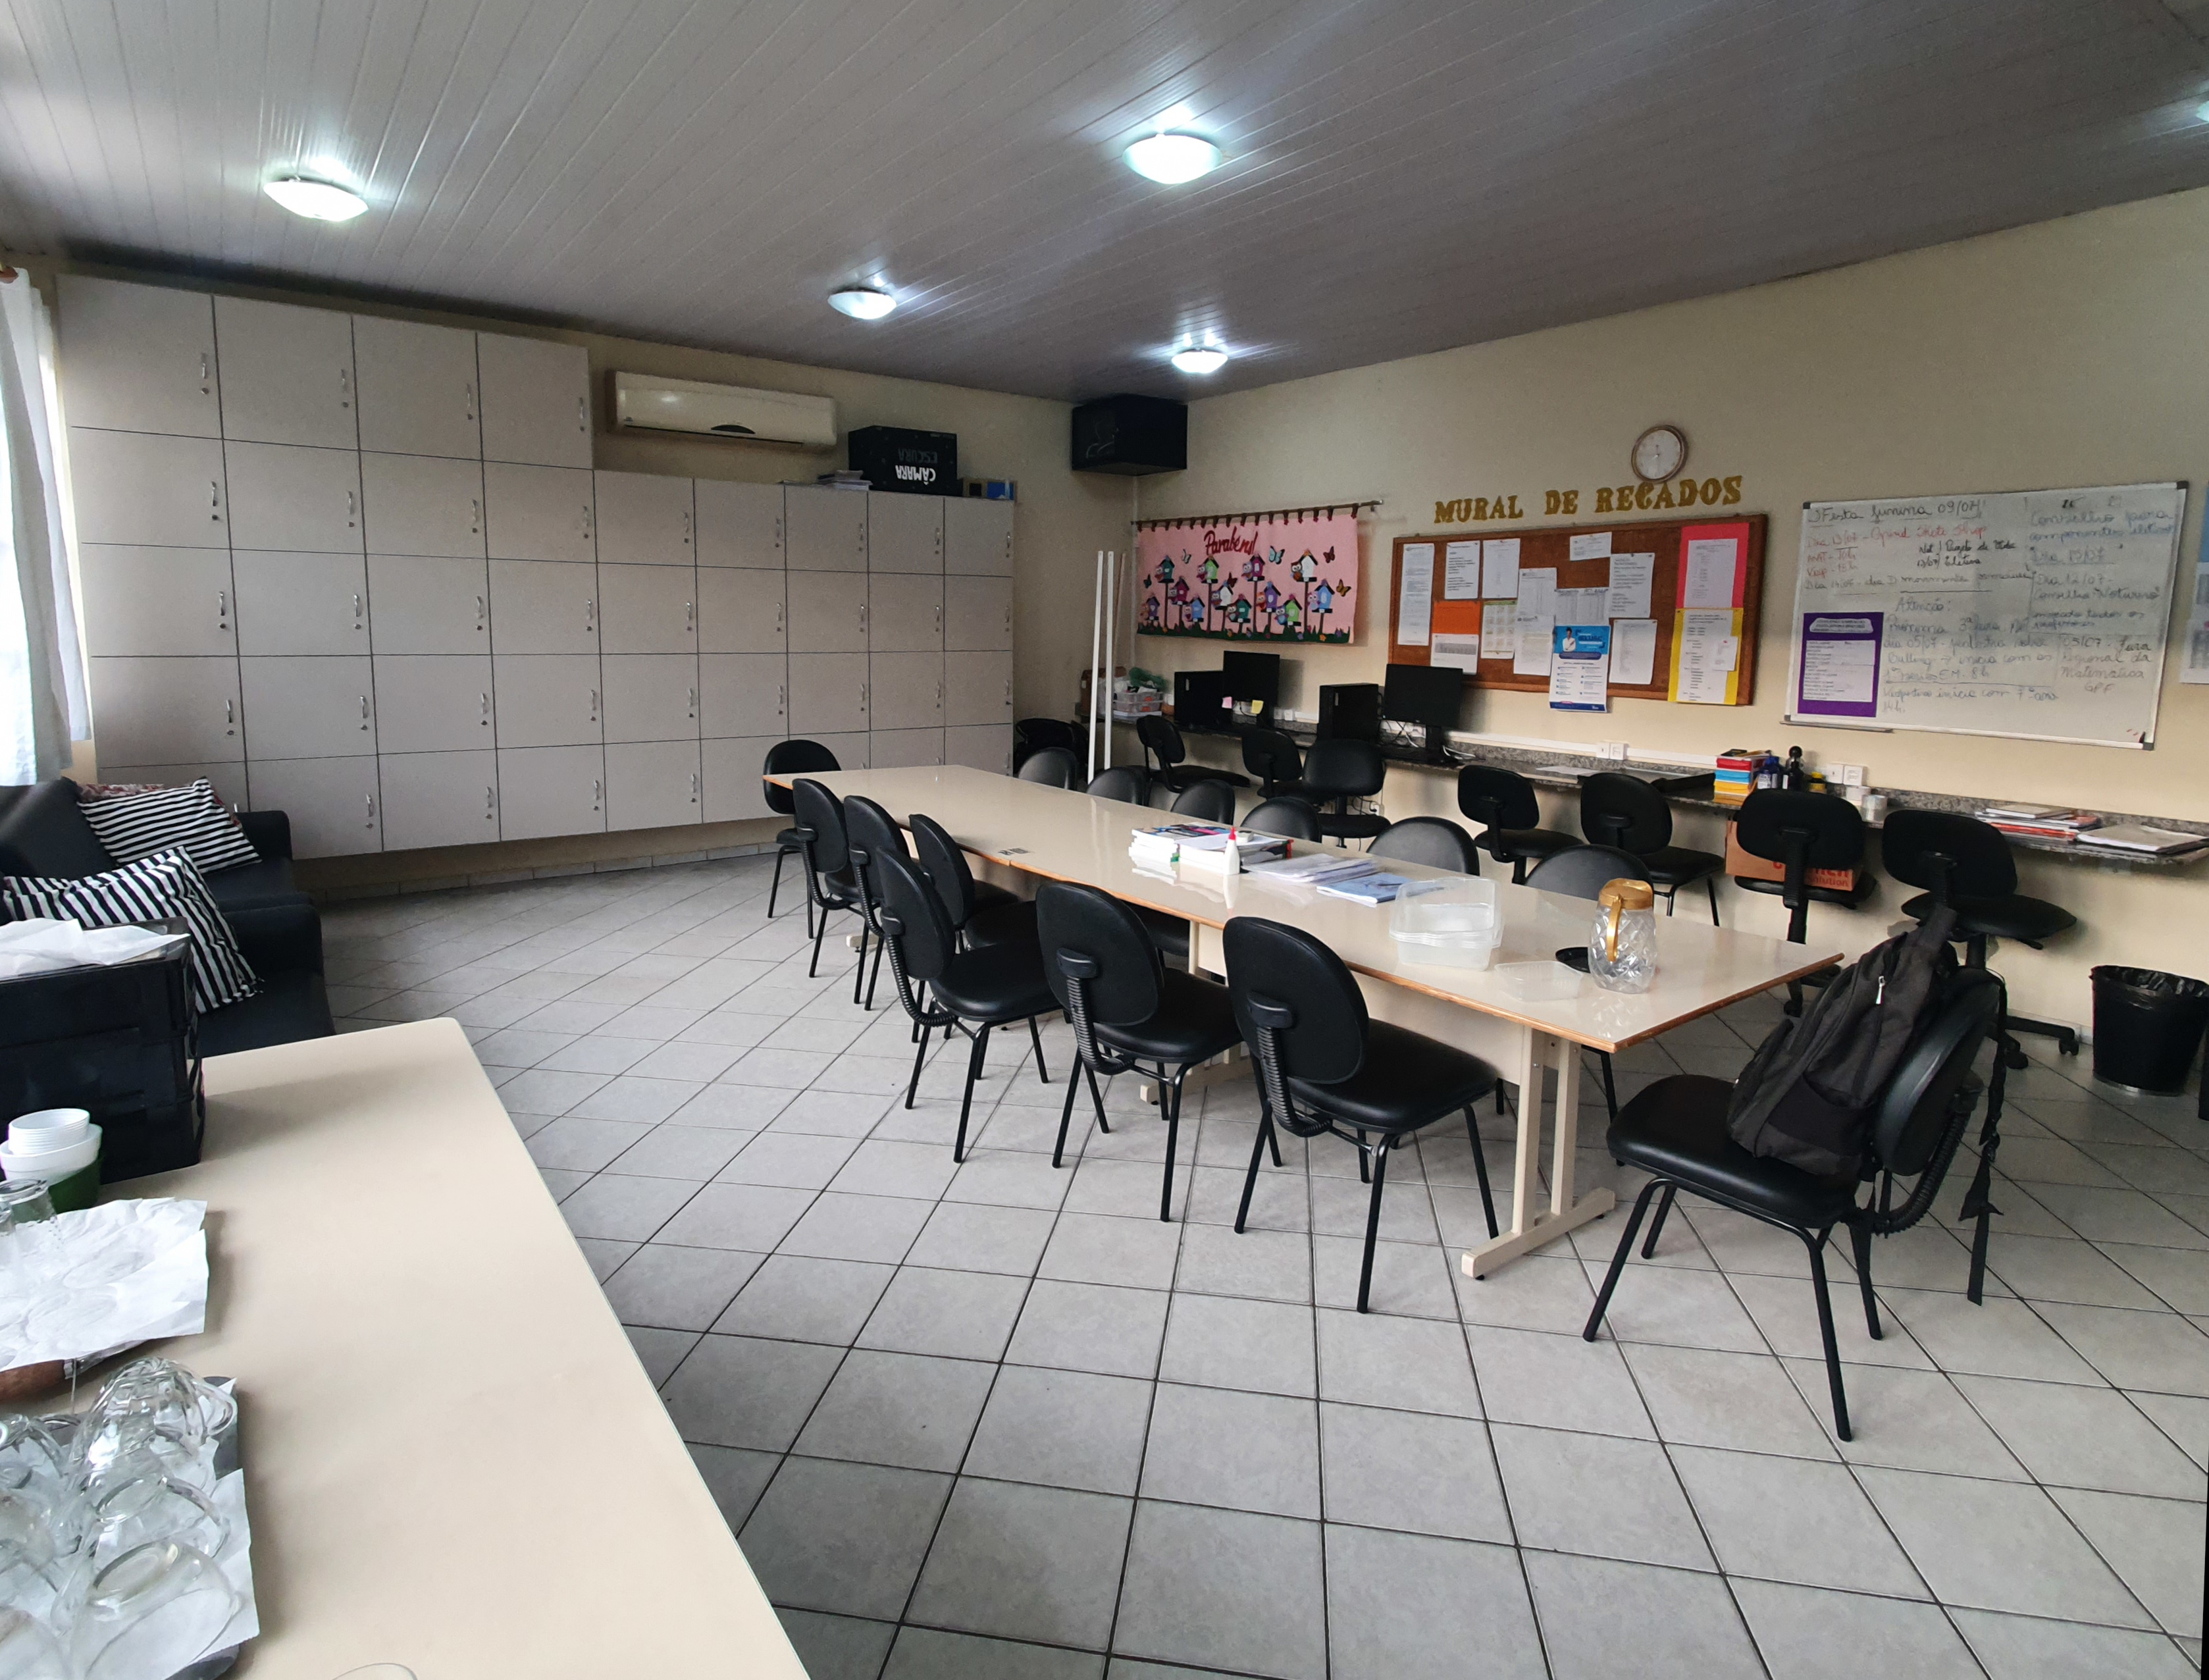
\includegraphics[width=.45\textwidth]{assets/sala-prof.jpg}
	\caption{Sala dos Professores}
	\label{fig:sala-prof}
\end{wrapfigure}
A Sala dos Professores, \autoref{fig:sala-prof}, possui: geladeira, forno de micro-ondas, aparelho de ar-condicionado e um purificador de água. É equipada com dois desktops conectados à internet. Cada professor tem um espaço nos armários e é nele que fica guardado o \emph{Data-Show} para uso em aulas diferenciadas.
% section Sala dos Professores (end)

\section{Laboratório} % (fold)
\label{sec:Laboratório}
As aulas experimentais podem ser conduzidas no Laboratório, preparado para atender as disciplinas de Física, Química e Biologia. Comporta cerca de 40 alunos e é composto por duas grandes bancadas e alguns armários. Há nele matériais para experimentos de cinemática, física dilatação térmica e eletrostática.
% section Laboratório (end)

\section{Laboratório de Informática} % (fold)
\label{sec:Laboratório de Informática}
\setlength\intextsep{0pt}
\begin{wrapfigure}[8]{l}{0.45\textwidth}
	\centering
	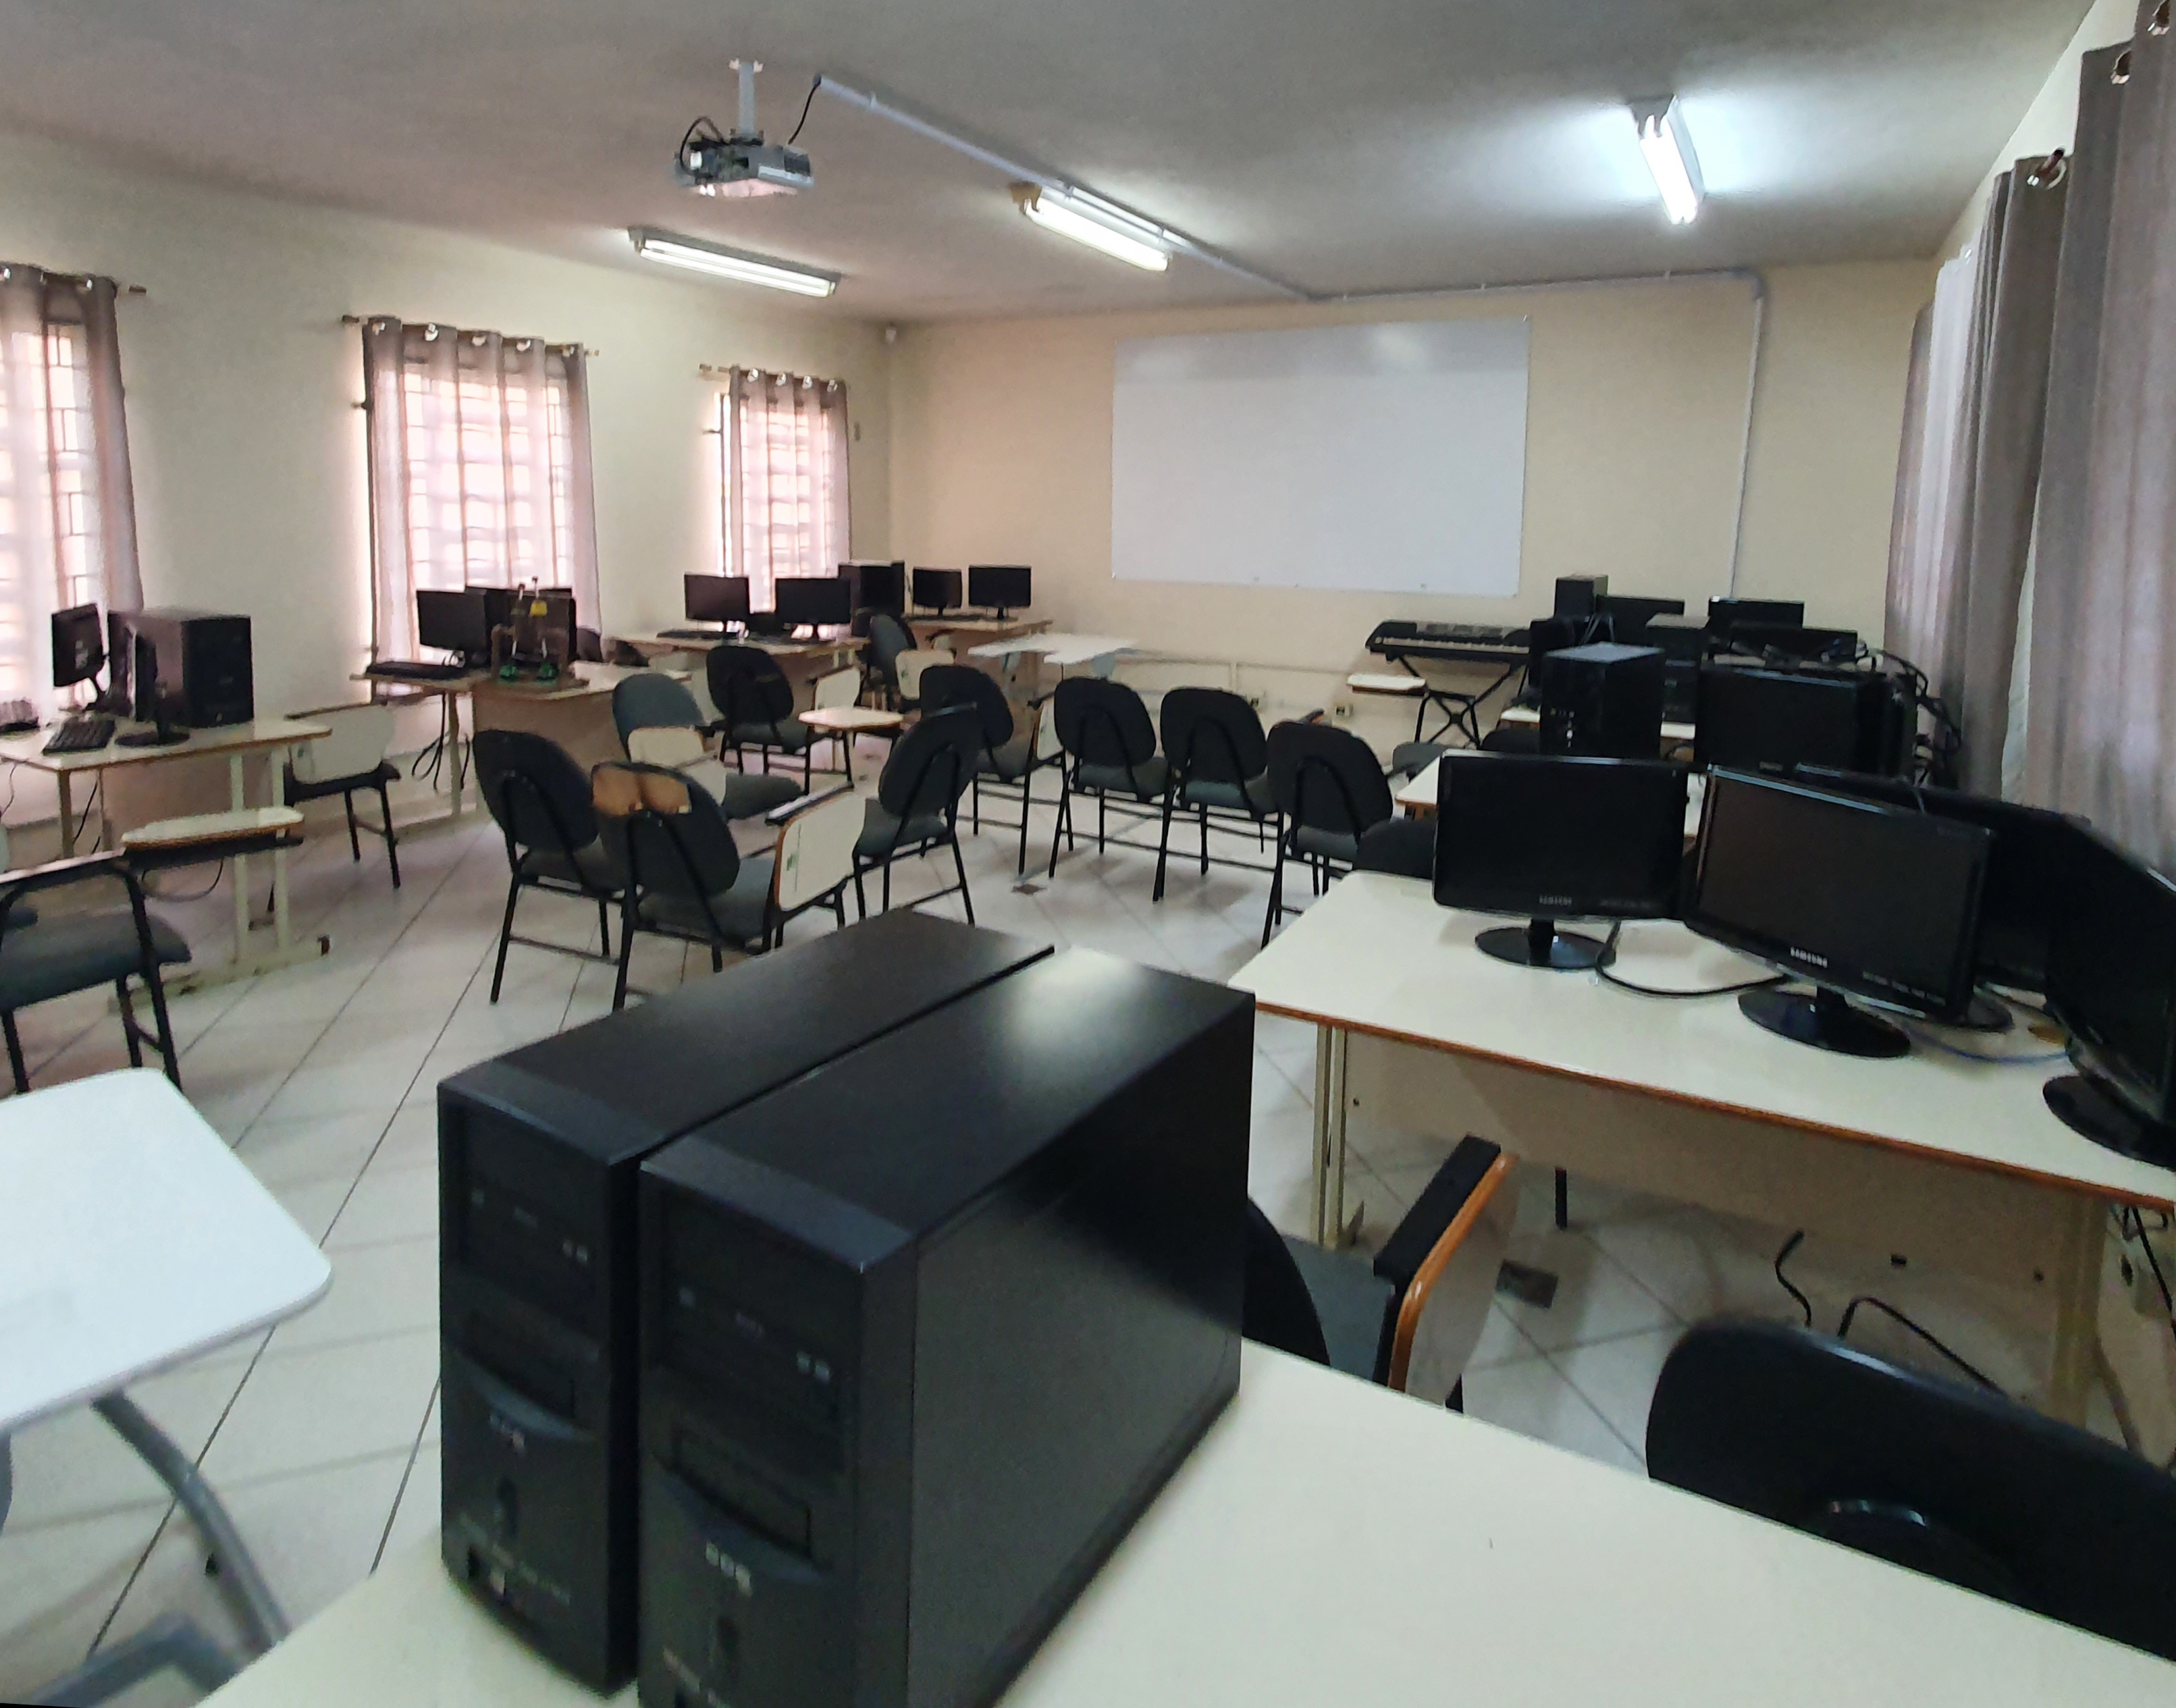
\includegraphics[width=.4\textwidth]{assets/sala-de-informatica02.jpg}
	\caption{Laboratório de Informática}
	\label{fig:sala-informatica}
\end{wrapfigure}
O Laboratório de Informática, \autoref{fig:sala-informatica}, é composto por nove desktops e dezenove monitores com acesso à internet, tem capacidade para atender até dezenove alunos em virtude da quantidade de dispositivos. Possui ainda uma Lousa Melamínica ($350\times 120$)\cm\; e retroprojetor.
% section Laboratório de Informática (end)

\section{Sala de Aula} % (fold)
\label{sec:Sala de Aula}
As Salas de Aulas são planejadas para comportar, em média, trinta alunos. Boa parte das salas possui aparelho de ar-condicionado, armários e são devidamente equipadas com Lousa Melamínica ($400\times 120$)\cm.
% section Sala de Aula (end)

\section{Auditório} % (fold)
\label{sec:Auditório}
\setlength\intextsep{0pt}
\begin{wrapfigure}[12]{r}{0.5\textwidth}
	\centering
	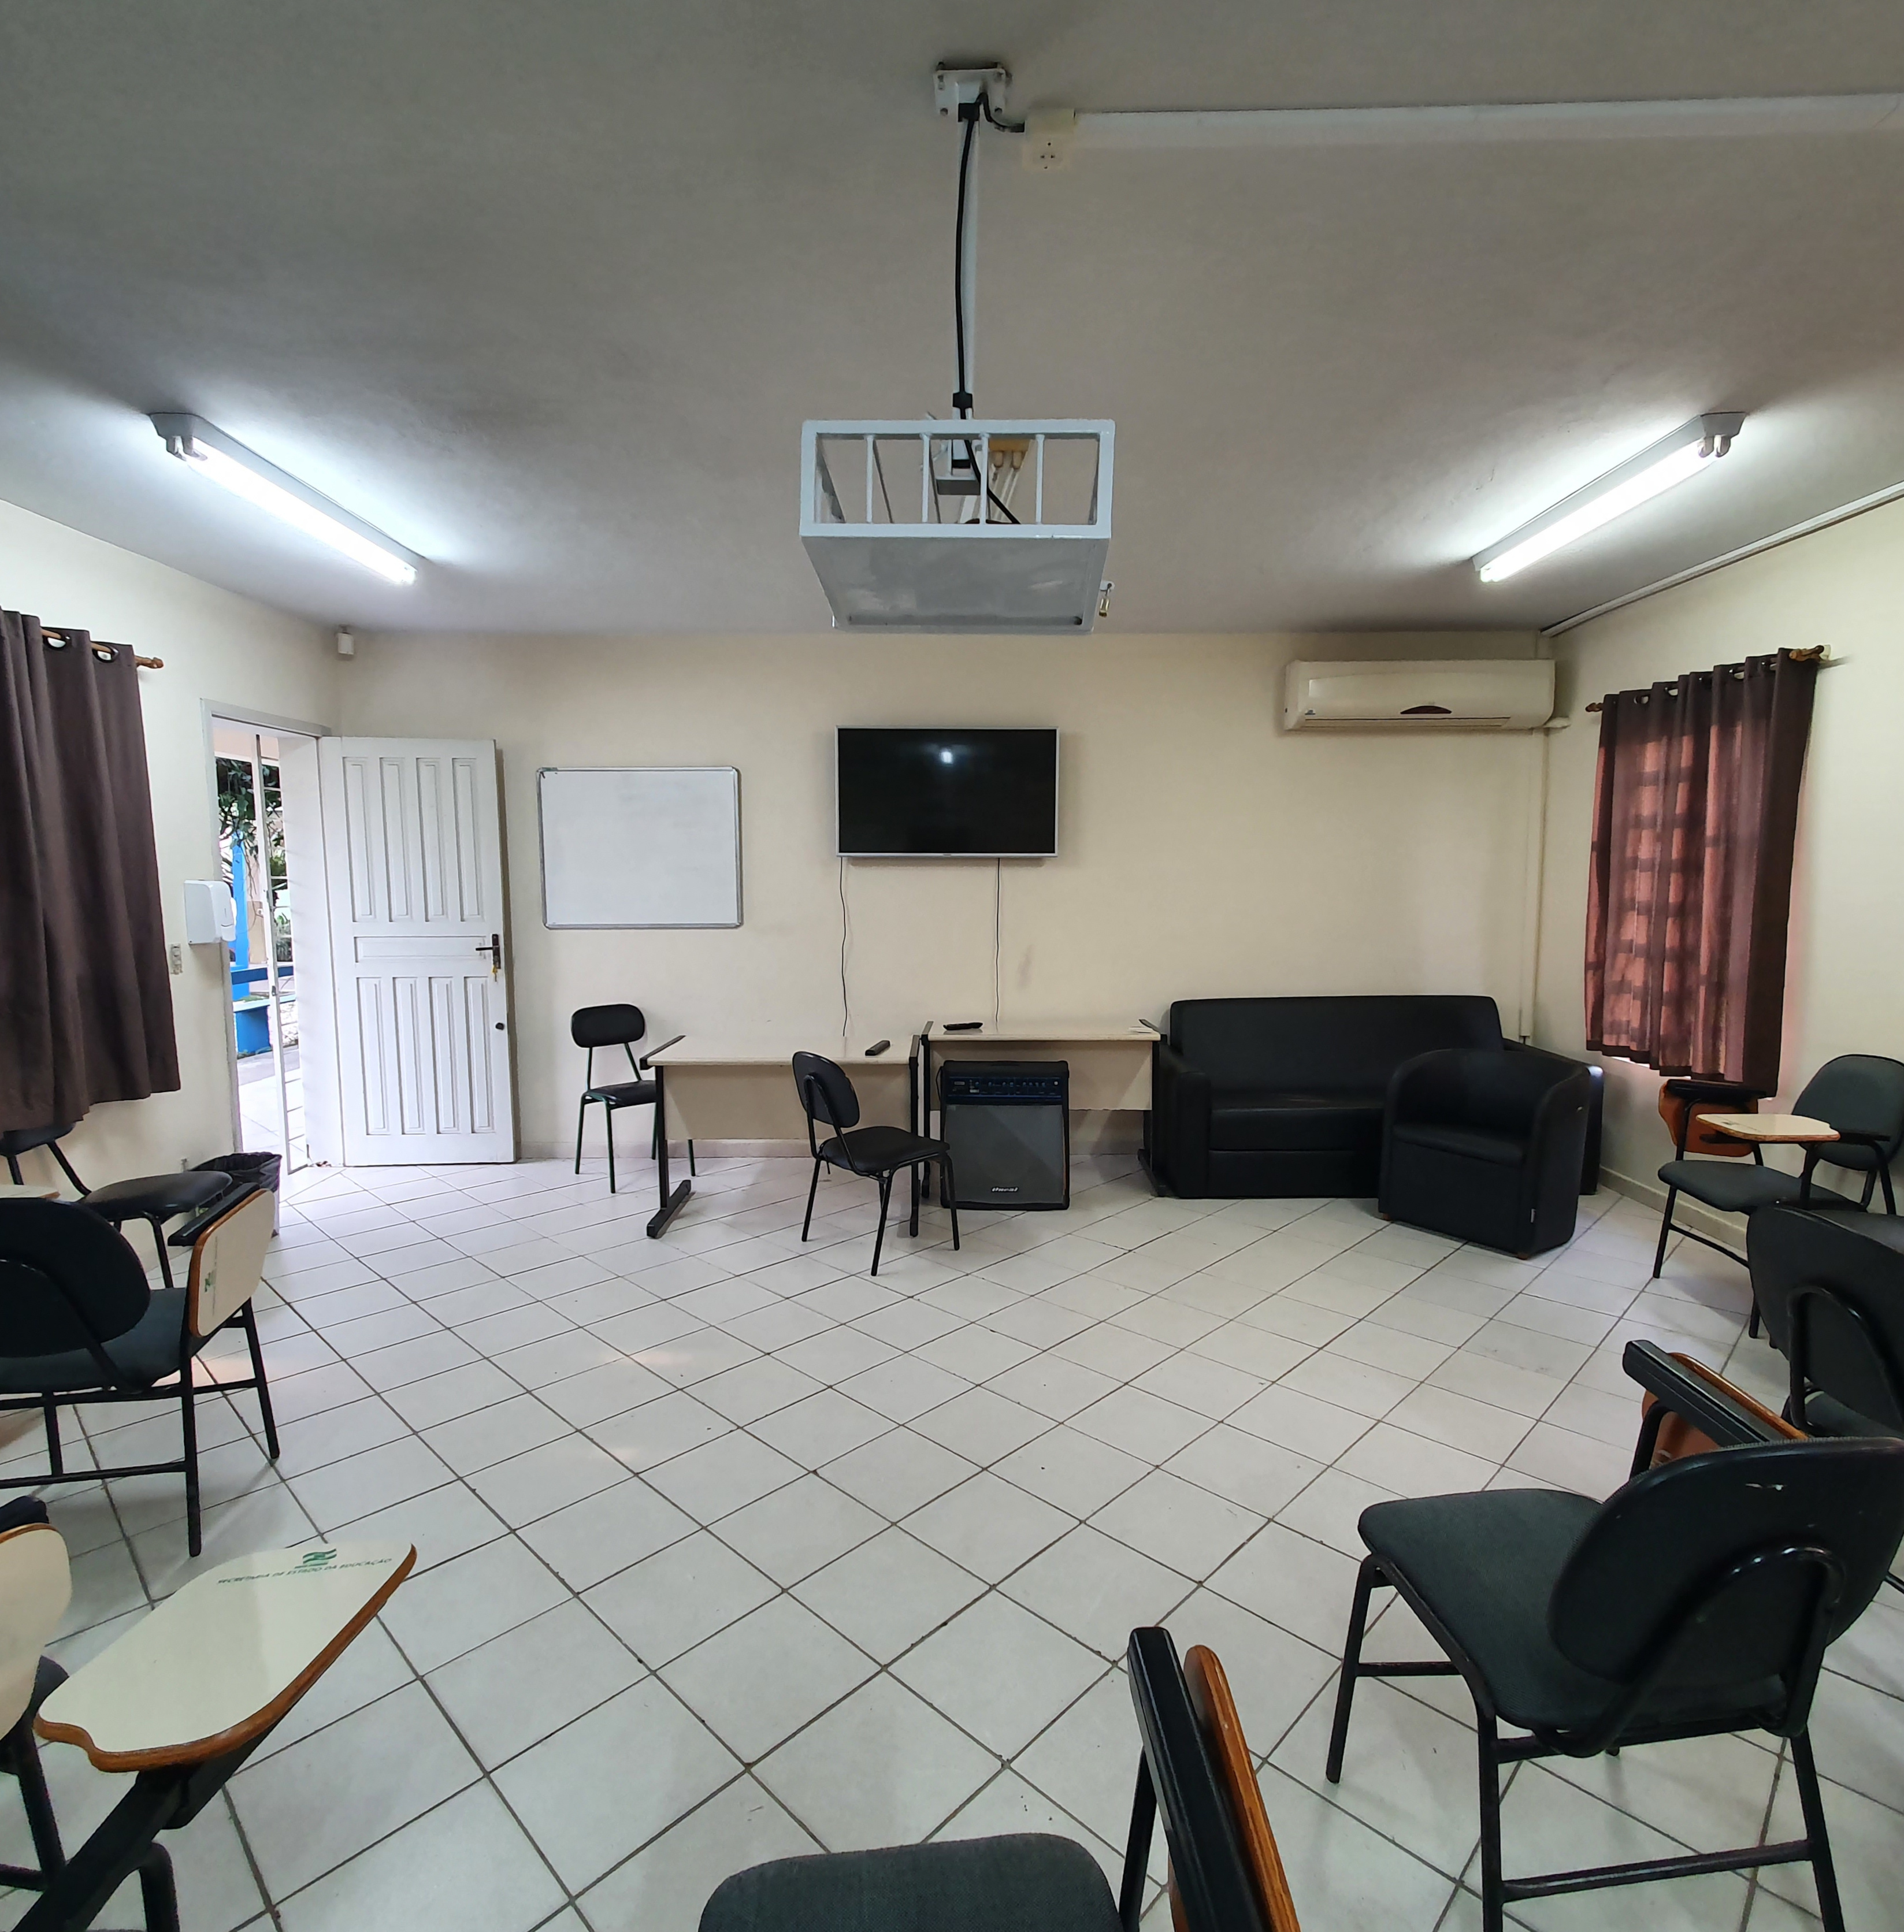
\includegraphics[width=.45\textwidth]{assets/auditorio-01.jpg}
	\caption{Auditório}
	\label{fig:auditorio-01}
\end{wrapfigure}
O auditório, \autoref{fig:auditorio-01}, tem capacidade para comportar um total quarenta pessoas e é equipado com um televisor de led $40\inch$, caixa de som amplificada multi-uso Oneal-OCM modelo 550 de $80\Watt$ de potência rms, um retroprojetor e ar-condicionado.
% section Auditório (end)

\section{Biblioteca} % (fold)
\label{sec:Biblioteca}
No acervo da Biblioteca, \autoref{fig:biblioteca-01}, encontram-se livros didáticos de todas as disciplinas, livros de literatura nacional e internacional, almanaques, \acp{DVD} educativos, revistas de assuntos dos mais variados e jornais. Possui também uma televisão de $32\inch$ a tubo conectada à uma leitora de \ac{DVD}, mesas e cadeiras o suficiente para comportar uma pequena turma de 10 pessoas.
\vspace{10pt}

\begin{figure}[ht!]
	\centering
	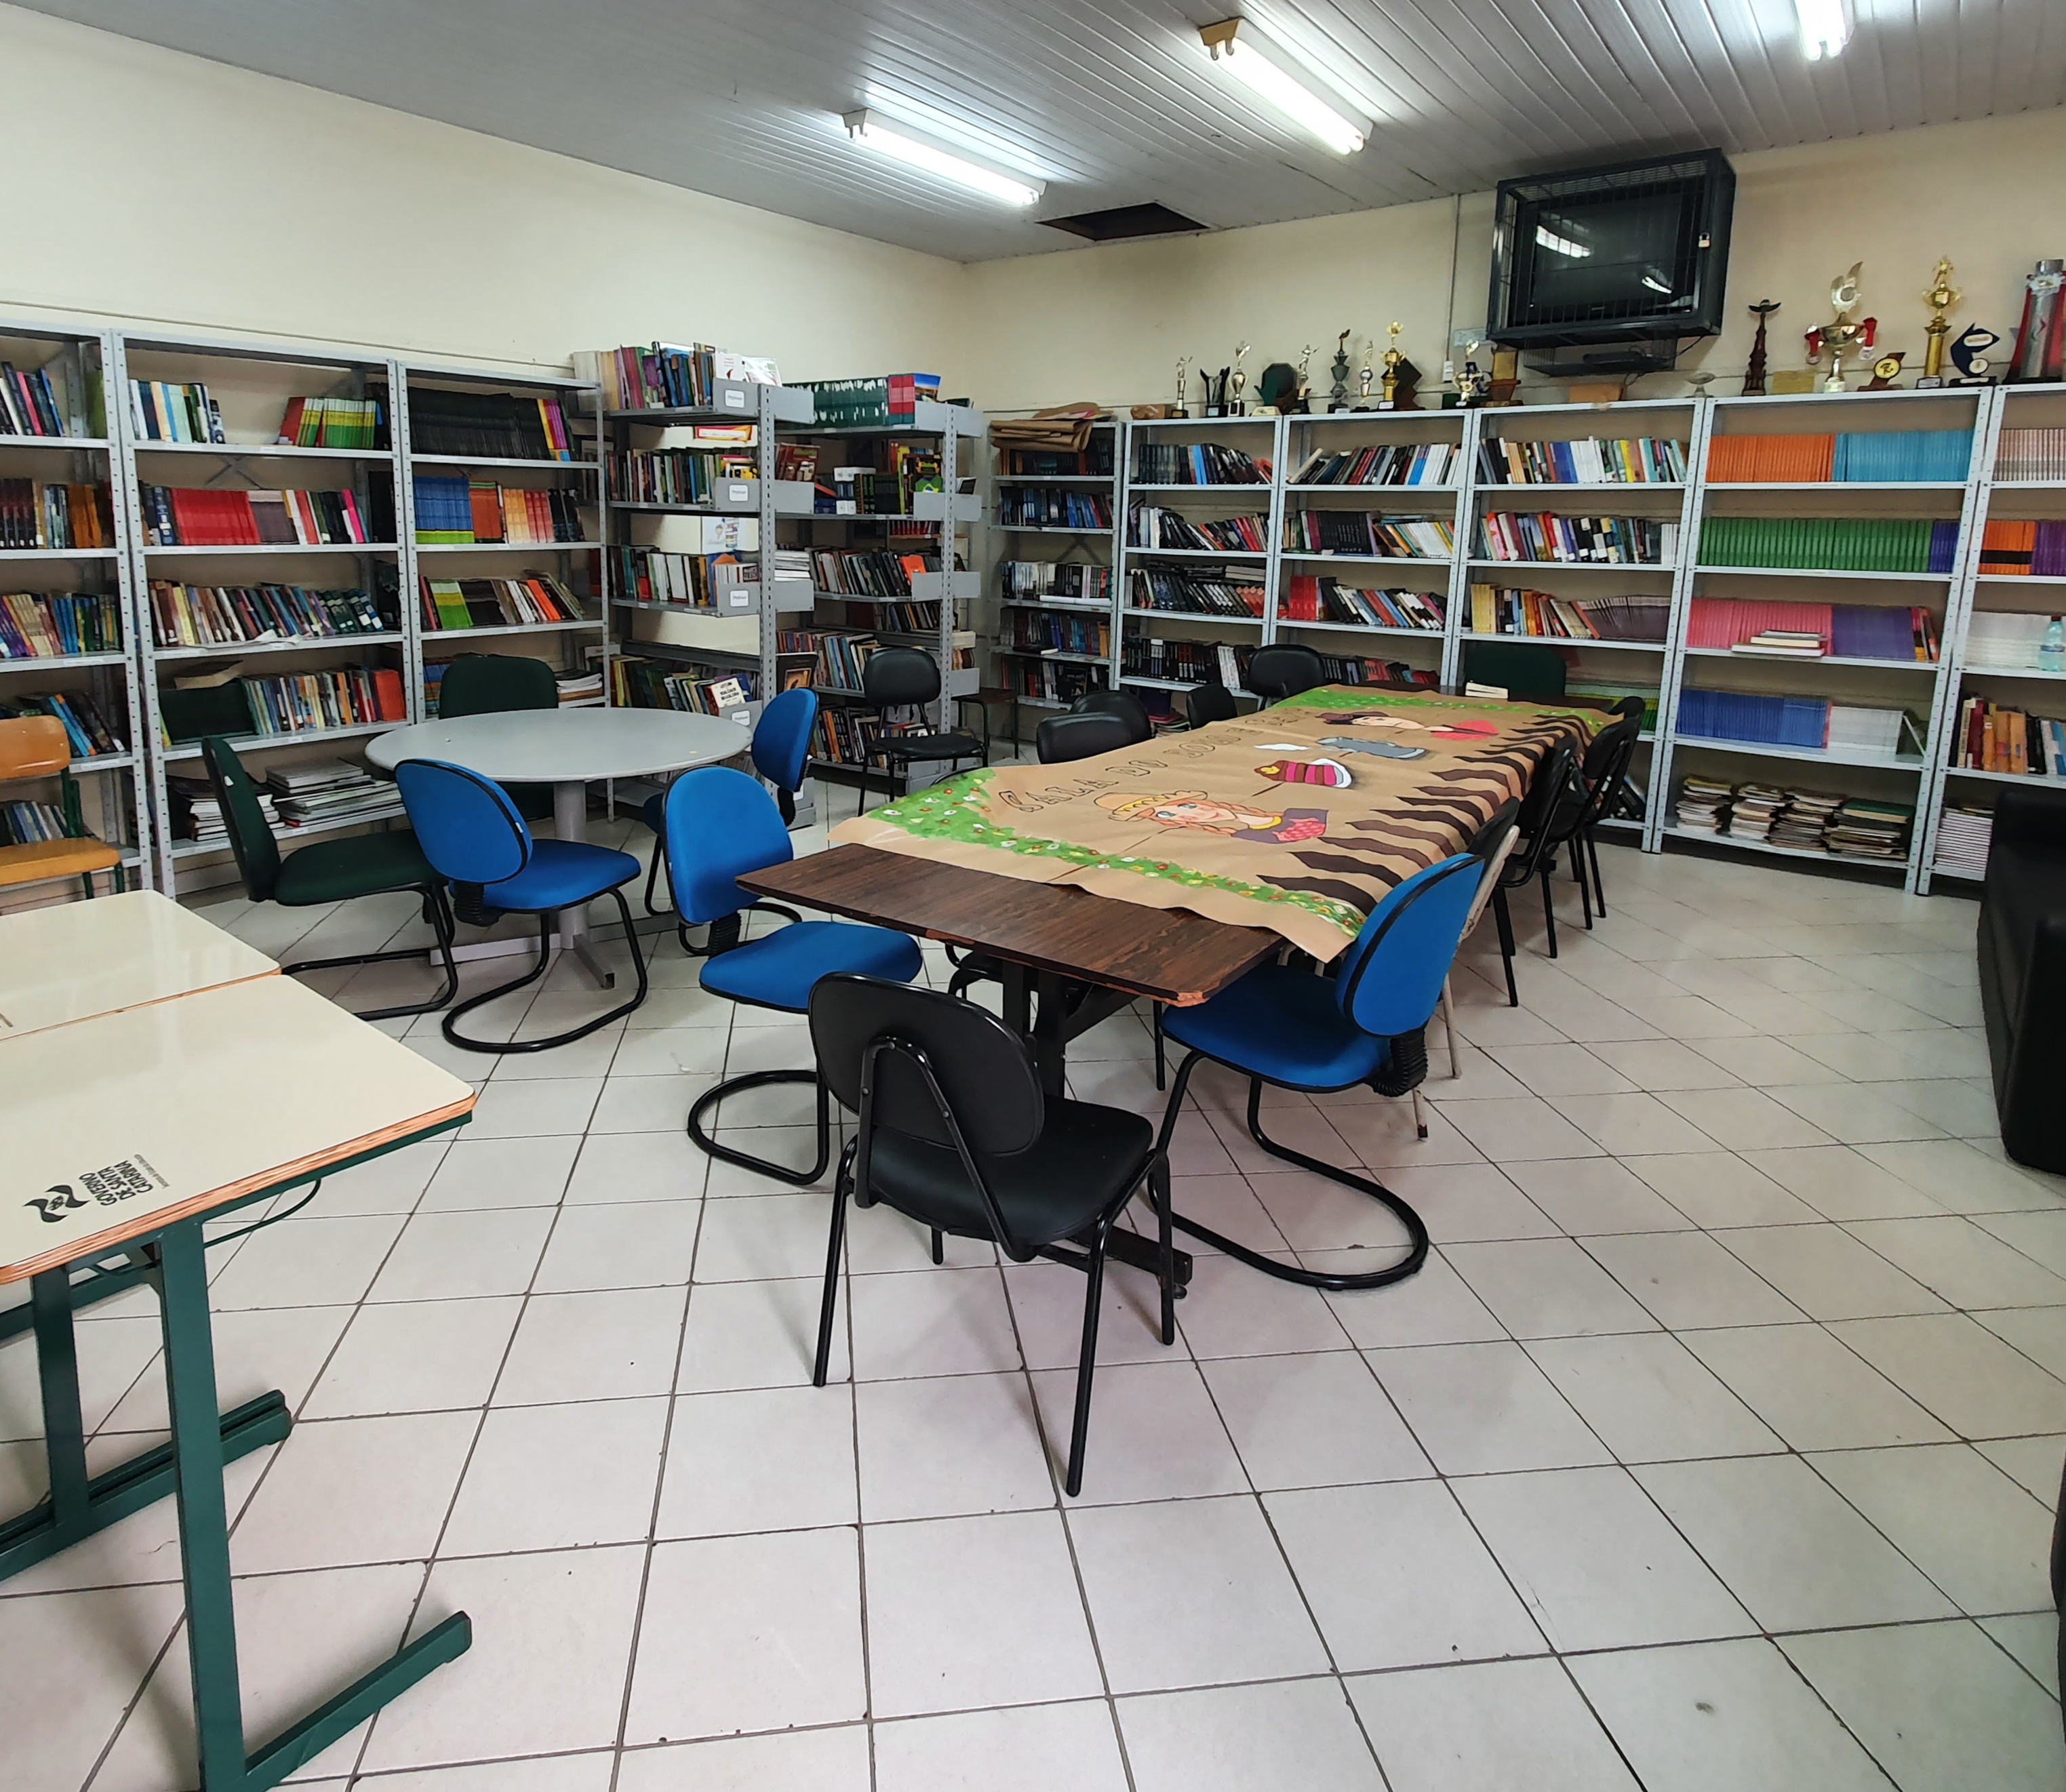
\includegraphics[width=.7\linewidth]{assets/biblioteca-01.jpg}
	\caption{Biblioteca}
	\label{fig:biblioteca-01}
\end{figure}
% section Biblioteca (end)

\section{Lousa Digital} % (fold)
\label{sec:Lousa Digital}
\setlength\intextsep{0pt}
\begin{wrapfigure}[10]{l}{0.45\textwidth}
	\centering
	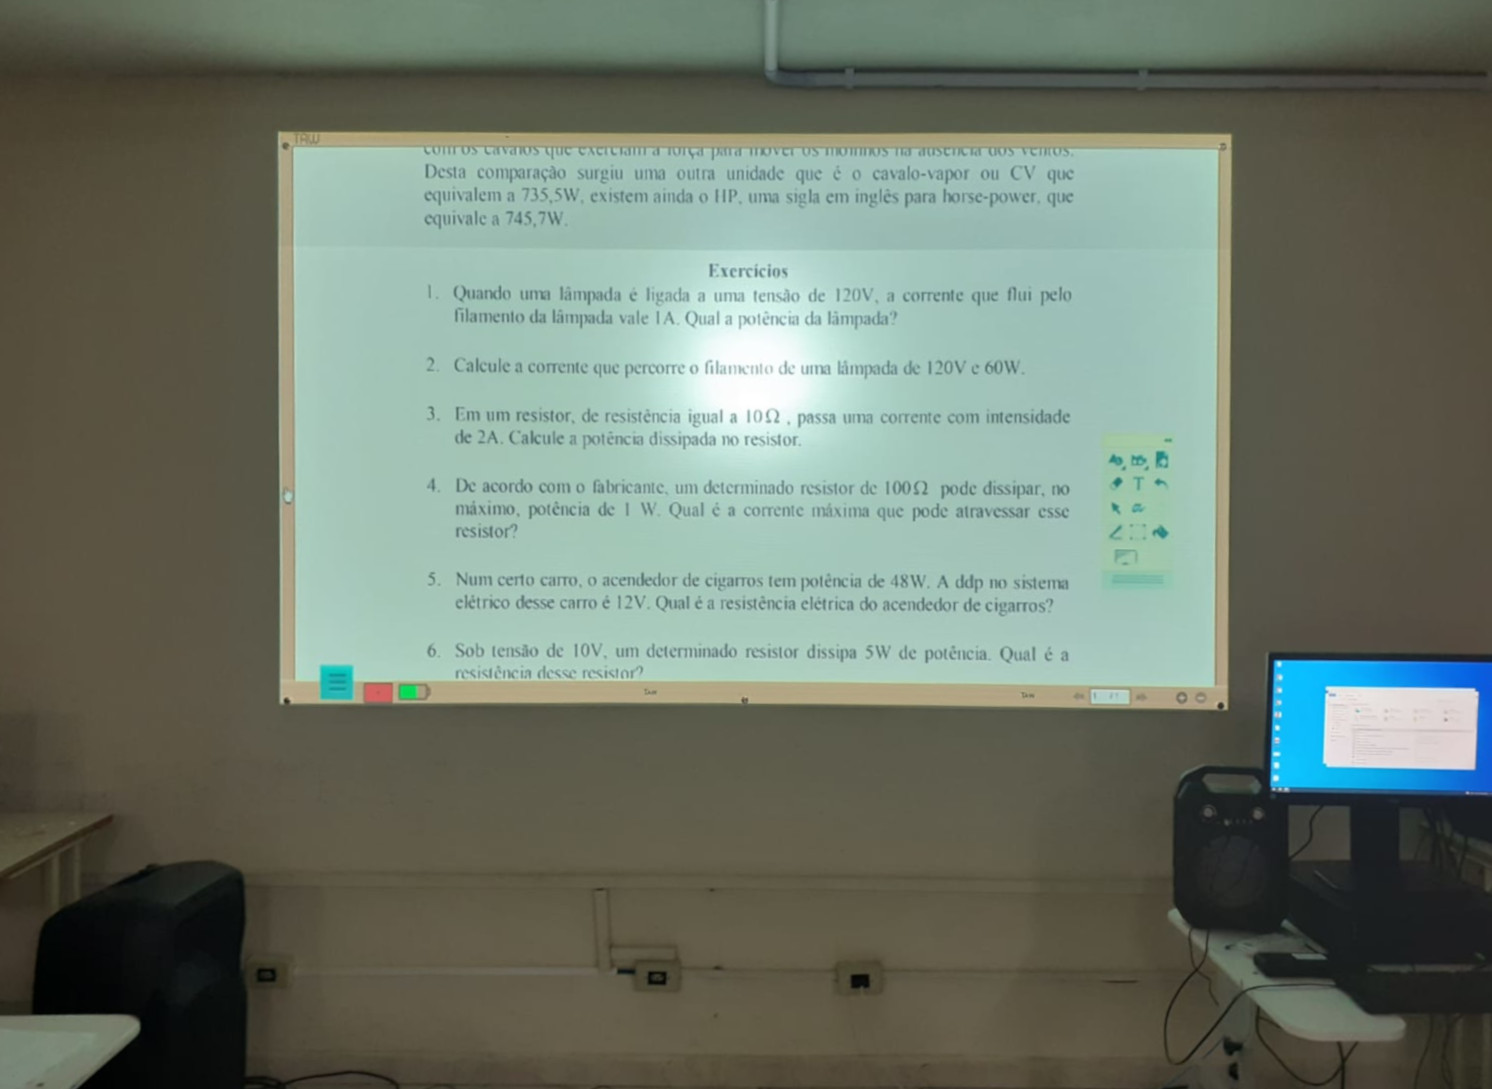
\includegraphics[width=.4\textwidth]{assets/d-lousa.jpeg}
	\caption{Lousa Digital}
	\label{fig:lousa-d}
\end{wrapfigure}
Recentemente foi instalada uma lousa digital interativa em apenas uma sala de aula, \autoref{fig:lousa-d}, nela é possível mostrar simulações, vídeos, sons, GIFs etc. É um recurso que poucos professores utilizam no momento, por somente haver uma em toda a escola. A escola tem previsão de até o final do ano de 2023, todas as salas de aulas possuam o equipamento instalado. A lousa já possui todos os dispositivos necessários para o seu devido funcionamento, ficando a critério do professor a opção de levar ou não seu notebook ou que mais achar melhor para incrementar a aula.
% section Lousa Digital (end)

\section{Tablets} % (fold)
\label{sec:Tablets}
A unidade também possui 32 Tablets conectados à internet de 200 Mb e com o sistema operacional Android. Neles, o professor costuma usar o aplicativo \emph{Kahoot} em atividades diferenciadas. Para manter os tablets sempre com a bateria carregadas e prontos para uso, a escola utiliza o gabinete móvel de recarga, como pode ser visto na \autoref{fig:tablets}.
\vspace{10pt}

\begin{figure}[htb!]
	\centering
	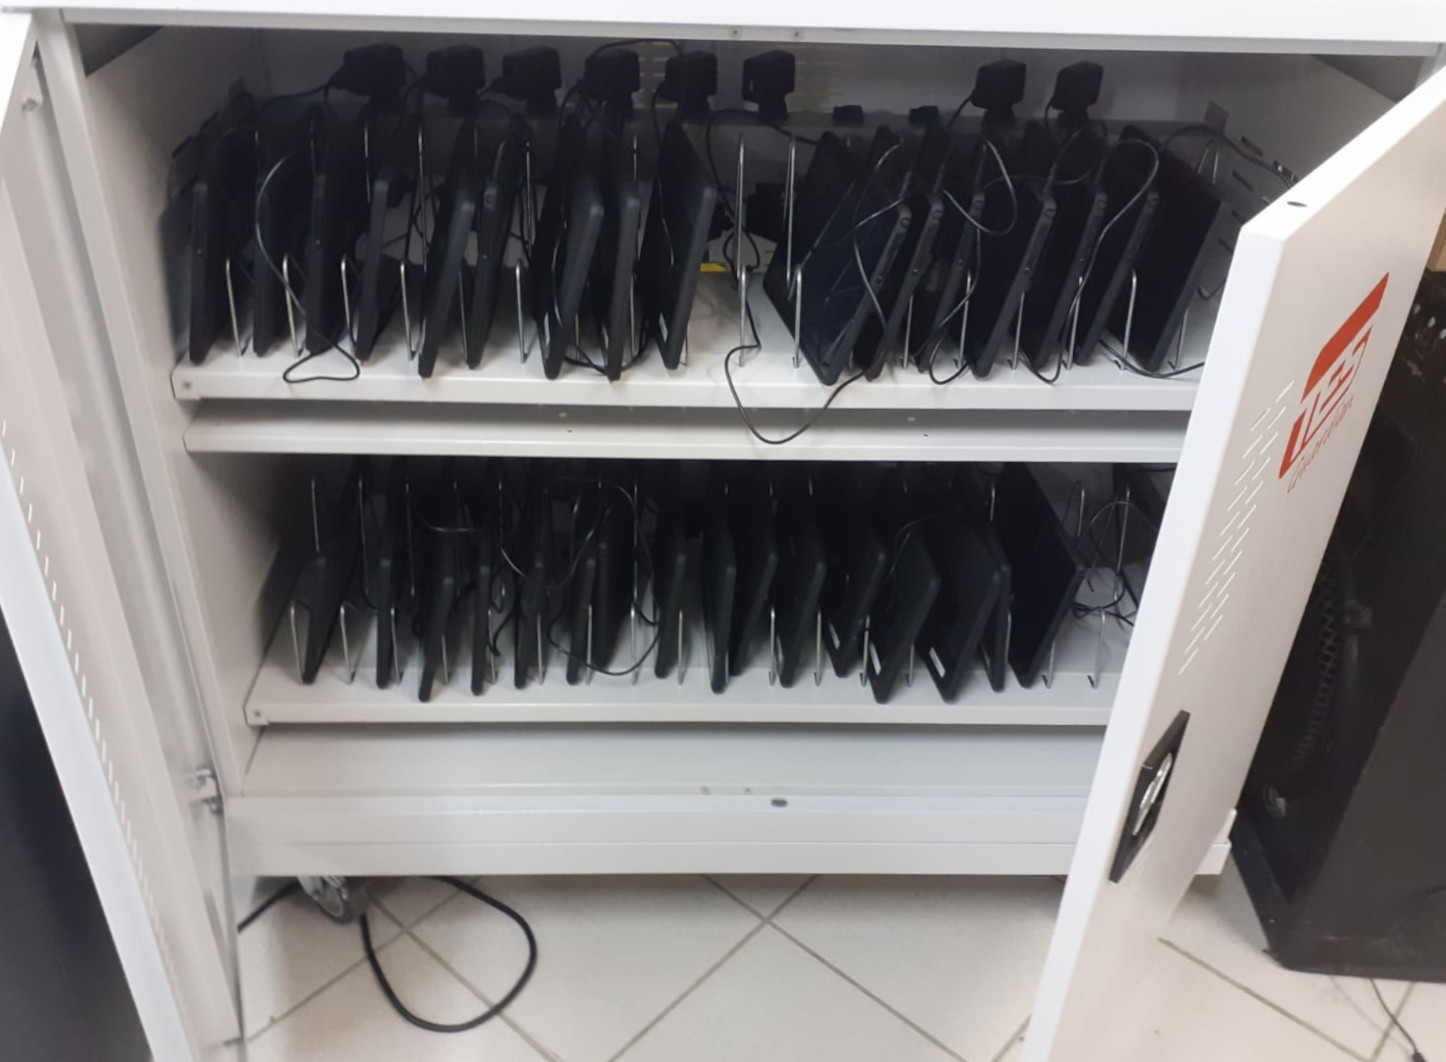
\includegraphics[width=.7\linewidth]{assets/tablets.jpeg}
	\caption{Tablets}
	\label{fig:tablets}
\end{figure}
% section Tablets (end)

% chapter Apoio à Docência (end)
